\documentclass{article}
\usepackage[margin=1in]{geometry}
\usepackage{graphicx}
\usepackage{amsmath}
\usepackage{booktabs}
\usepackage{tabularx}
\usepackage[colorlinks=true, urlcolor=blue, linkcolor=red]{hyperref}

\begin{document}
\section*{Analyzing Netflix's Strategic Shift Towards Diversity}

\subsection*{Introduction}

This project investigates Netflix's strategic shift towards diversity by analyzing the ethnic representation of actors over time. By showing the diversity index of actor's ethnicities and of the production countries and creating visualizations, we aim to demonstrate the increasing inclusivity in Netflix's casting choices. We also aim to show the shift in content, but with only the description to analyze, sufficient conclusions were not made.

\noindent The analysis process is shown in the Jupyter Notebook in our \href{https://github.com/cparthiv/RHS-TSA-Data-Science-Qualifier-2024}{Github repository}.

\subsection*{Methodology and Tech}

\noindent\textbf{Ethnicity Inference}: Removed duplicate names and used a model trained on US census and voter data from the \texttt{ethnicolr} library to predict ethnicities based on names, and chose the race with the highest probability. \newline
\noindent\textbf{Calculating Diversity Index}: the Simpson diversity index was used throughout this analysis.




\subsection*{Visualizations}

\begin{figure}[h!]
    \centering
    \begin{minipage}[t]{0.65\textwidth}
        \vspace{0pt} % Aligns the top of the figure with the text
        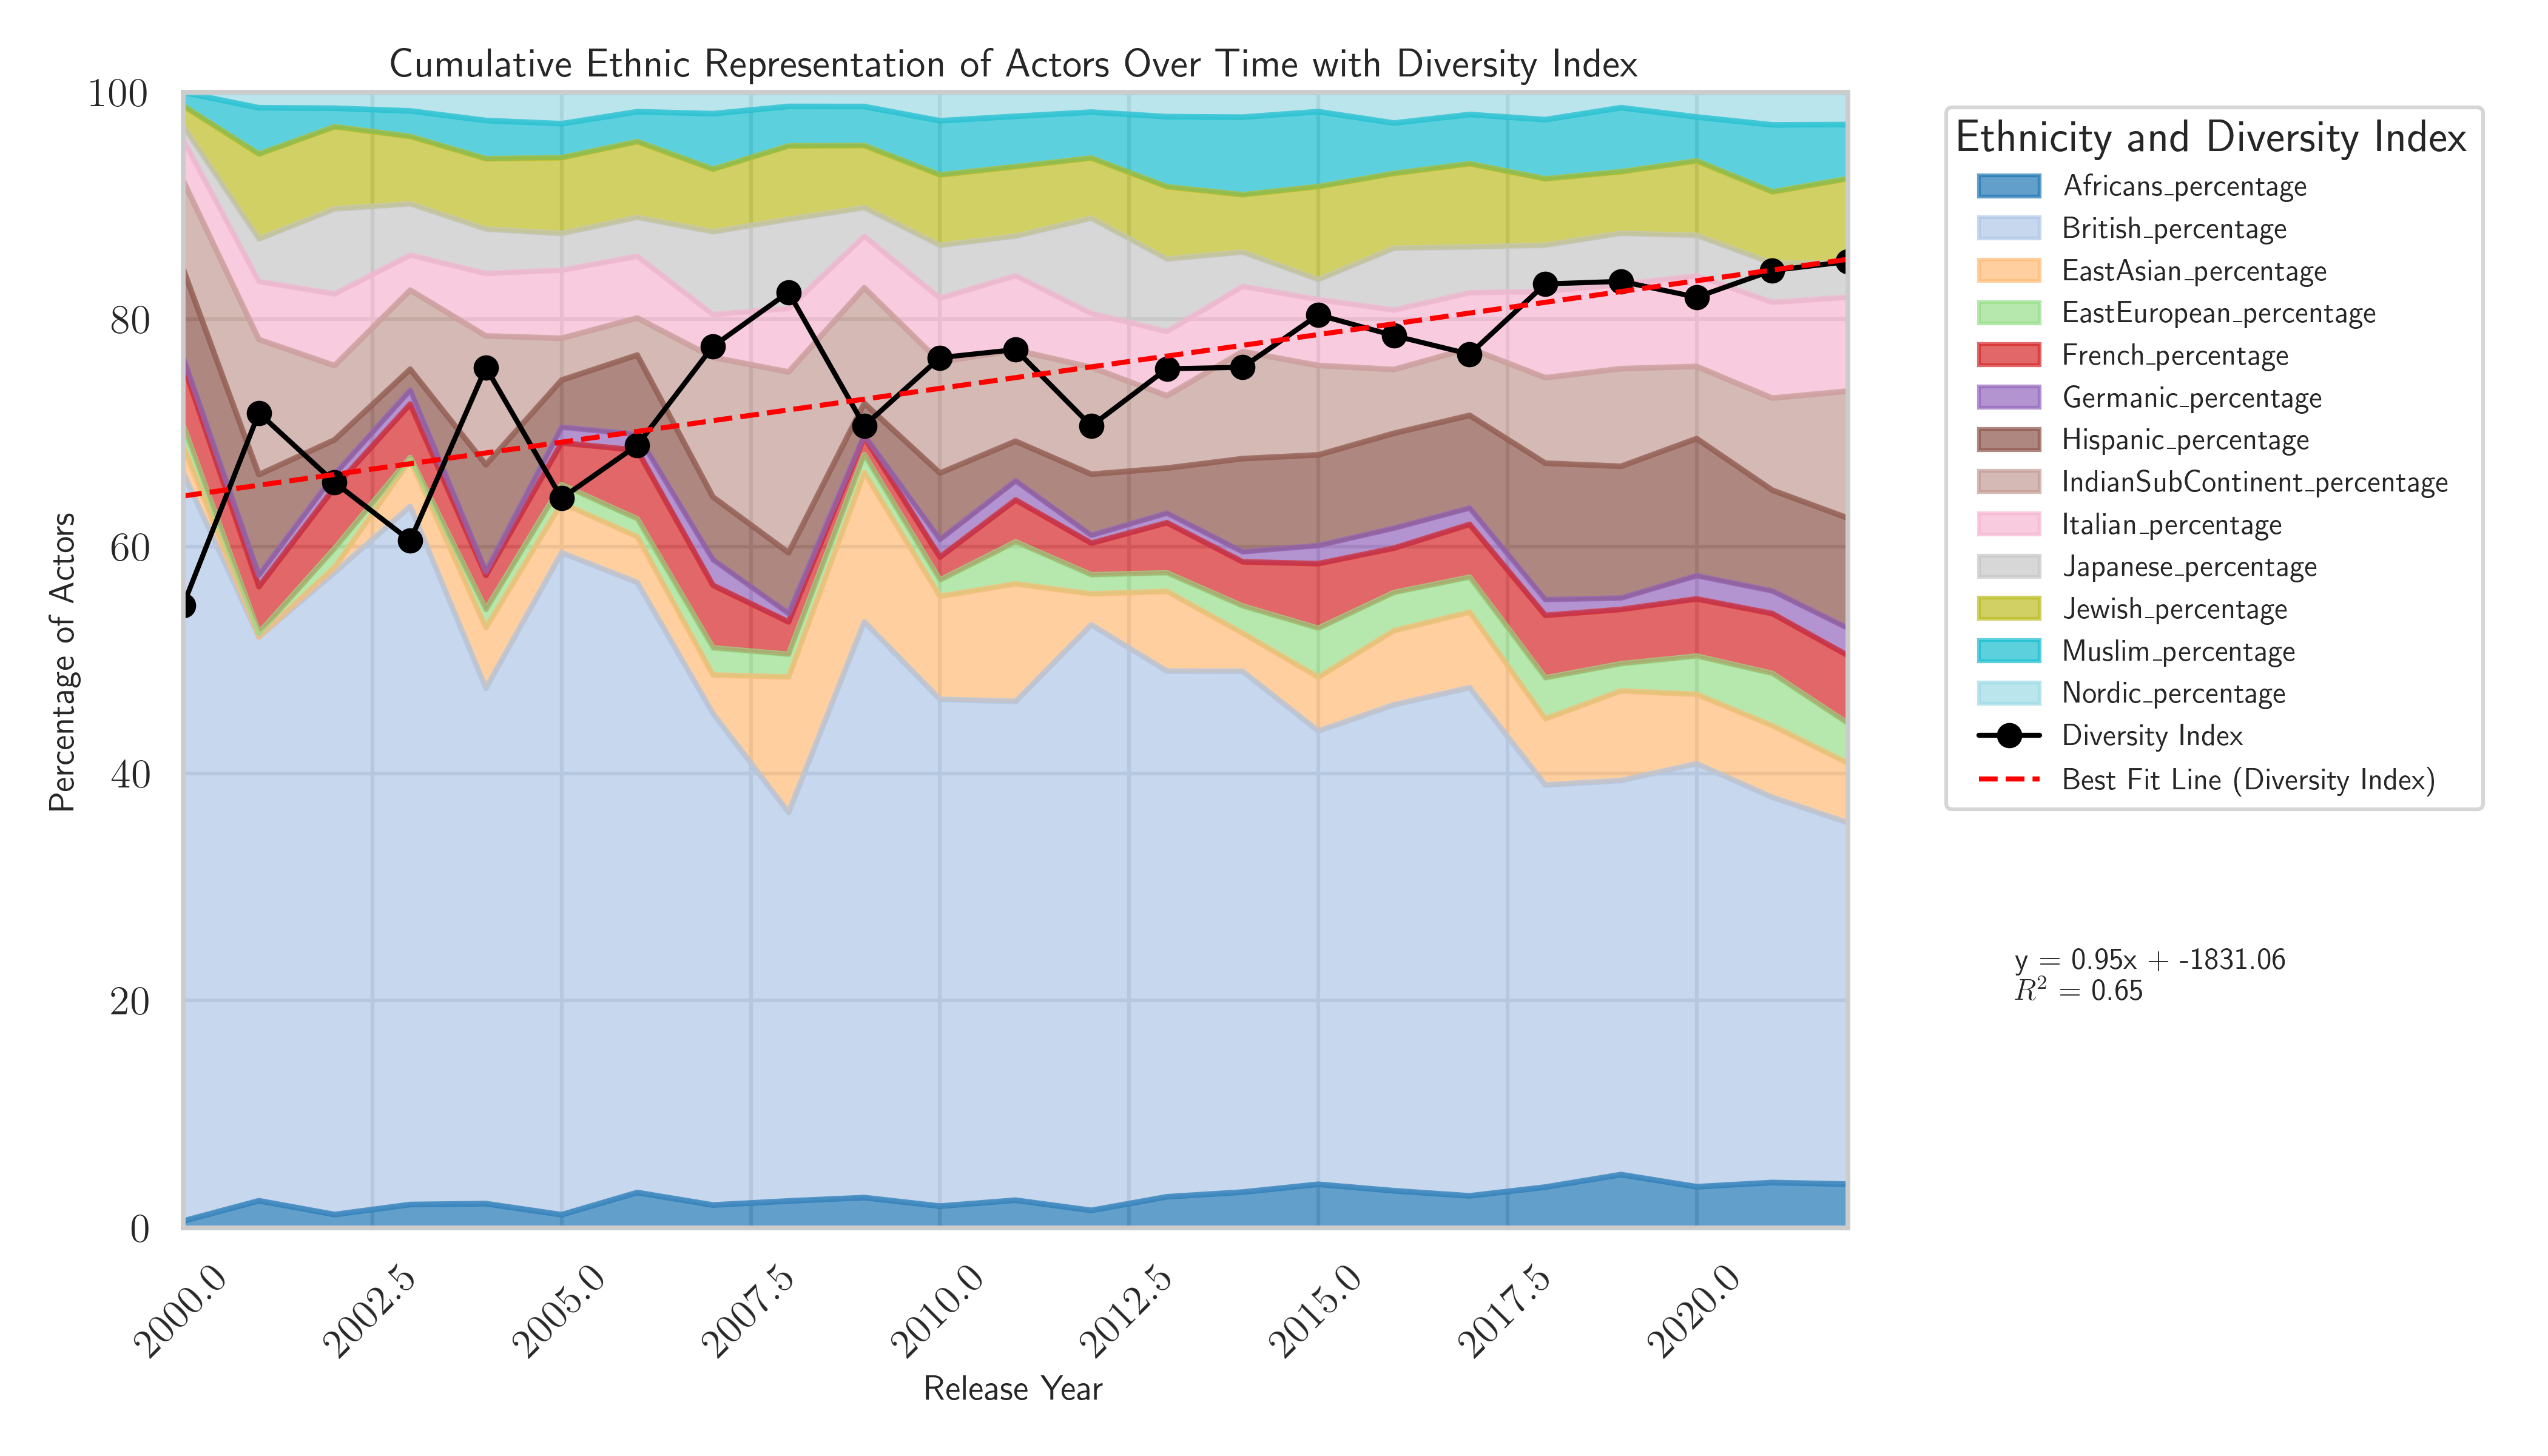
\includegraphics[width=\linewidth]{ethnicity_area_chart_with_best_fit.png}
        \label{fig:ethnicity-area-chart}
    \end{minipage}%
    \hspace{0.6cm} % Adjusts horizontal space between figure and text
    \begin{minipage}[t]{0.3\textwidth}
        \subsubsection*{1. Ethnic Representation Over Time}

        An area chart was created to show the cumulative ethnic representation of actors from 2000 to 2022.\newline
        The diversity index was overlaid as a black line, with a red dashed best fit line representing the trend. As annotated on the graph, the \(R^2\) value was 0.65, indicating a reasonably strong positive correlation.
    \end{minipage}
\end{figure}


\begin{figure}[h!]
    \centering
    \begin{minipage}[t]{0.3\textwidth}
        \subsubsection*{2. Simpson Index of Production Countries Over Time}

        A line chart was created to display the Simpson Diversity Index of production countries. \newline
        The diversity trend is shown over time, providing insights into how Netflix has expanded their offerings. The fluctuations until around 1995 were caused by a small sample size, as Netflix typically streams newer titles, but afterwards there is a strong positive trend. 
    \end{minipage}
    \hspace{0.6cm} % Adjusts horizontal space between figure and text
    \begin{minipage}[t]{0.65\textwidth}
        \vspace{0pt} % Aligns the top of the figure with the text
        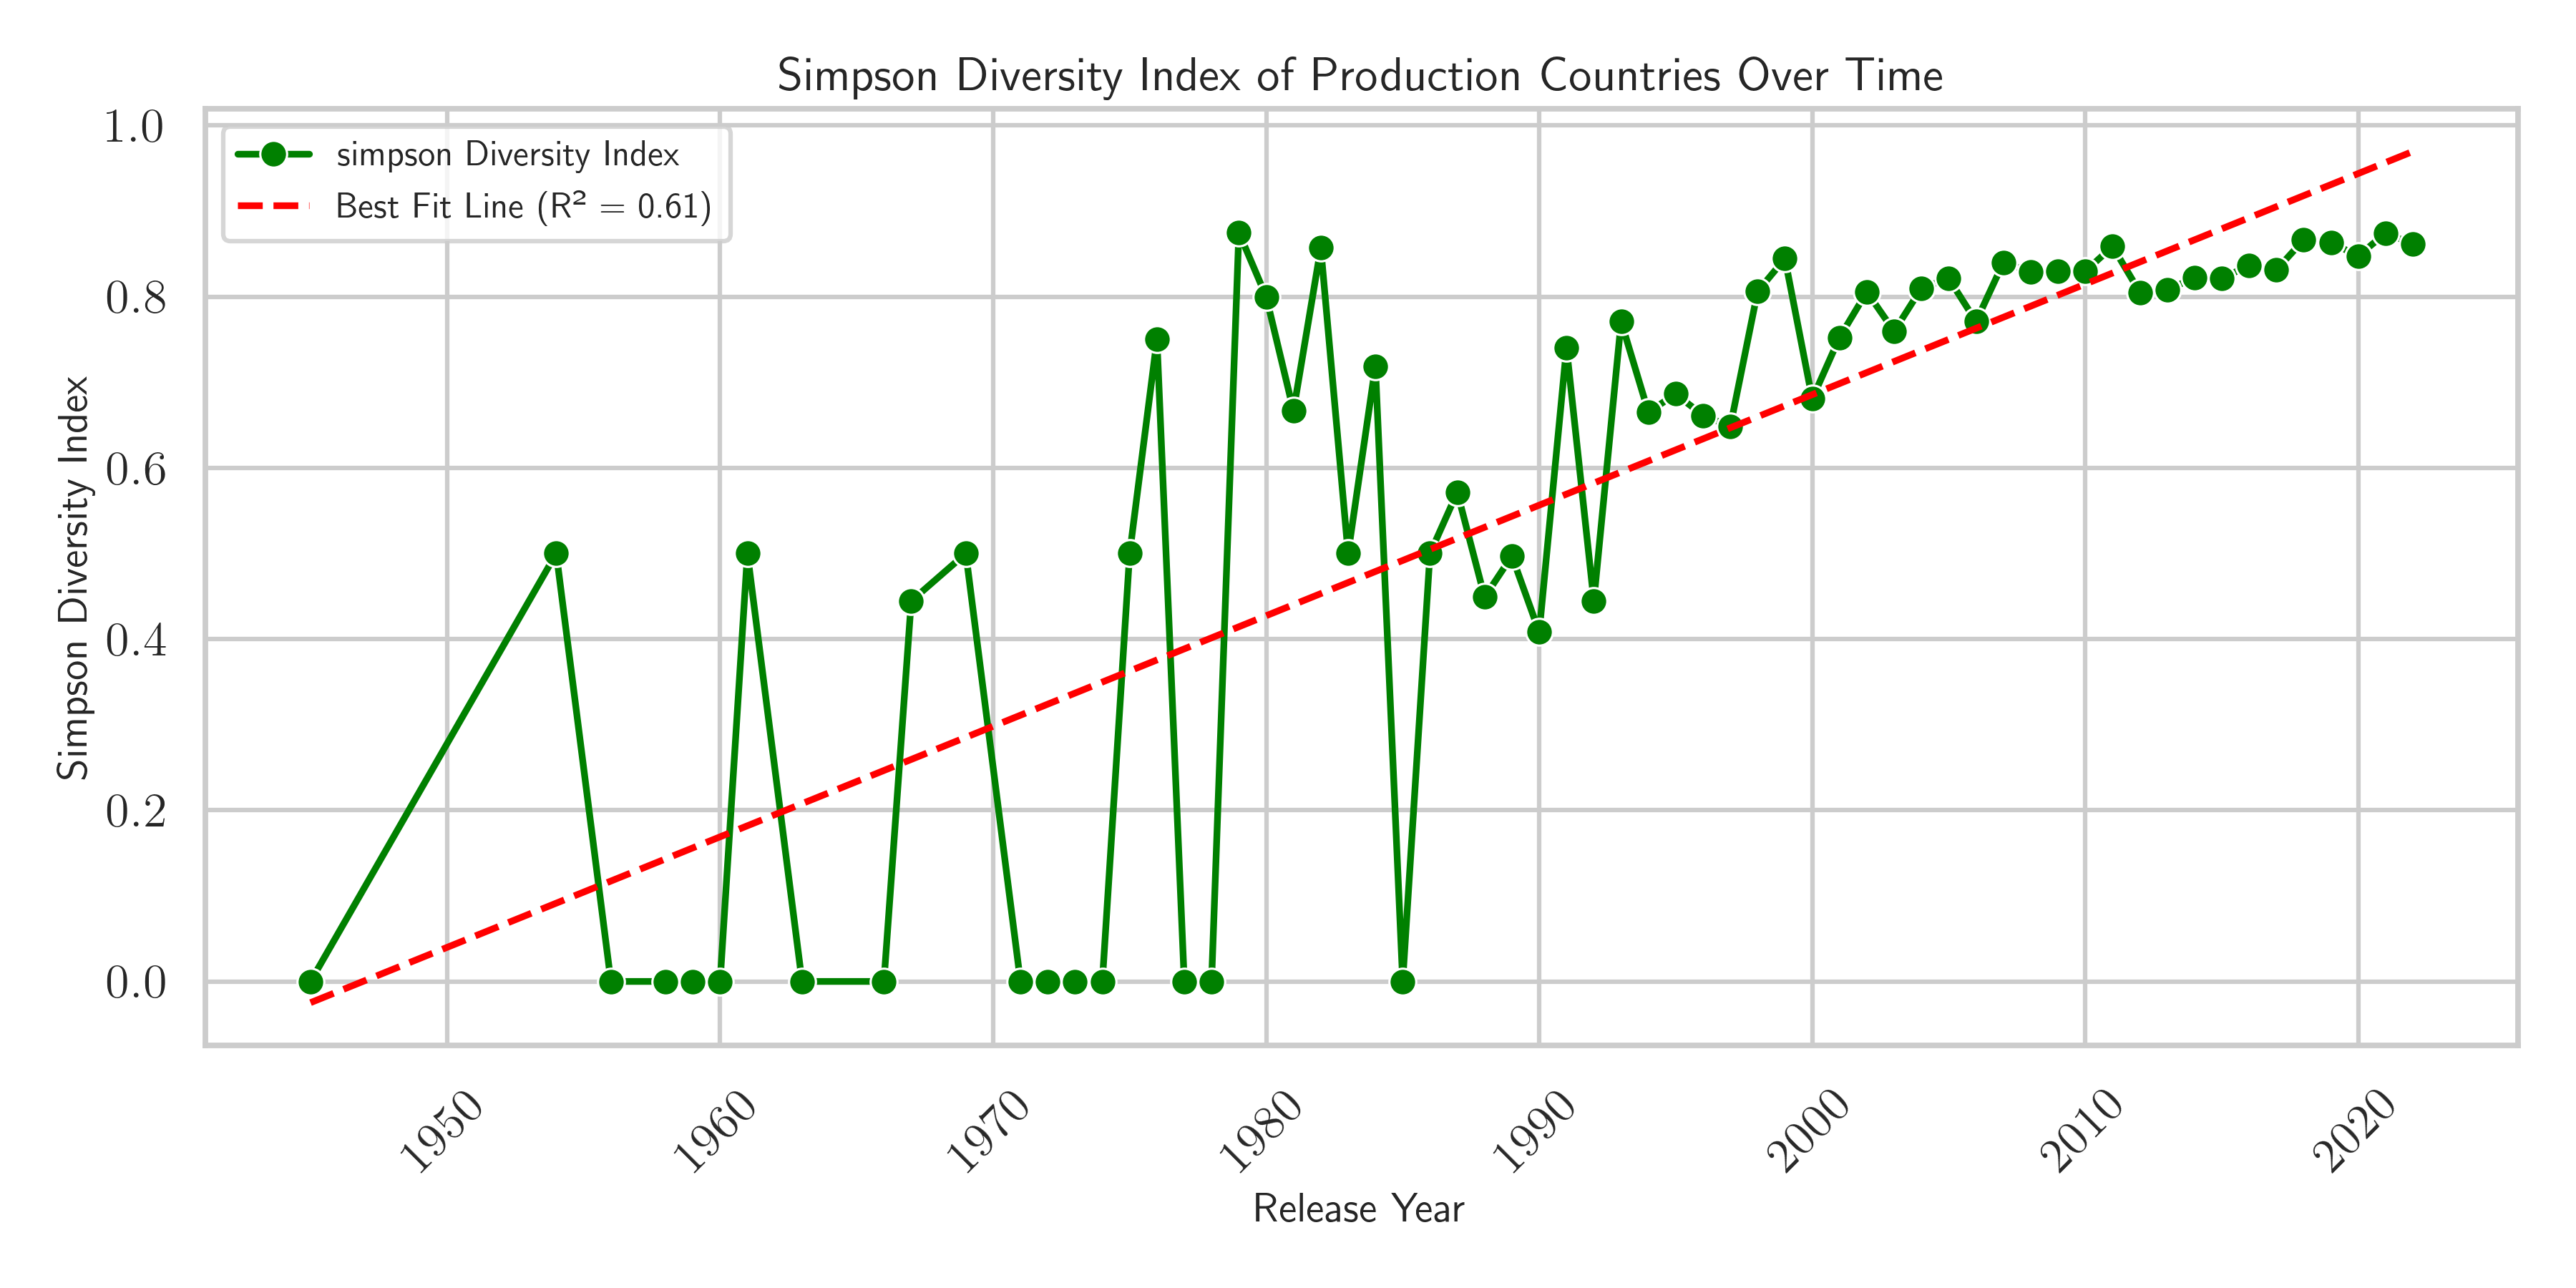
\includegraphics[width=\linewidth]{simpson_index_over_time.png}
        \label{fig:simpson-index-over-time}
    \end{minipage}%
    
\end{figure}



\end{document}
